% !TEX root = main.tex

\section{Symbolic execution of binary code}

The importance of performing symbolic analysis of a program's properties on binary code is on the rise for a number of reasons. Binary code analysis is attractive as it reasons on code that will actually execute: not requiring source code significantly extends the applicability of such techniques (to, e.g., common off-the-shelf proprietary programs, firmwares for embedded systems, malicious software), and it gives the ground truth important for security applications whereas source code analysis may yield misleading results due to compiler errors and optimizations~\cite{BITBLAZE-ICISS08}. Also, the recent advances in runtimes for programs written in dynamic languages brought just-in-time compilation to the masses, taking over on interpreters used when no efficient source-to-binary translation of code was statically possible. 

Analyzing binary code is commonly seen as a challenging task due to its complexity and lack of a high-level semantics\mynote{[D] I'm omitting obfuscation, code packing, and encryption for now}. Modern architectures offer complex instruction sets: modeling each instruction can be difficult, especially in the presence of multiple side effects on processor flags to determine branch conditions. The second major challenge comes from the lack of the higher-level semantics present in source code, especially when no debugging information is available. Types are not explicitly encoded in binary code: even with register types, it is common to store values from one type and read them as another. Similar considerations can be made for array bounds as well. Also, control-flow graph information is not explicitly available, as control flow is performed through jump instructions at both inter- and intra-procedural level. The function abstraction at the binary level does not exist as we intend it at source-code level: functions can be separated in non-contiguous pieces, and code may also call in the middle of a code block generated for a source-level function.

In the remainder of this section we provide an overview of how symbolic executors can address some of the most significant challenges in the analysis of binary code.

\subsection{Lifting to an Intermediate Representation}
Motivated by the complexity in modeling native instructions and by the variety of architectures on which applications can be deployed (e.g., x86, x86-64, ARM, MIPS), symbolic executors for binary code typically rely on a {\em lifter} that transforms native instructions into an {\em intermediate representation} (IR, also called {\em bytecode}) as those used in compilers. The inverse process is called {\em lowering} and is performed by a compiler when it generates native code for the IR obtained during the first step of compilation; IR is then compiled to native code for a specific platform. Source-code symbolic executors can resort to lowering performed by compilers to reason on bytecode rather than source-language statements\mynote{say something about Java}: for instance, ~\cite{KLEE-OSDI08} reasons on the IR generated by the LLVM compiler for static languages such as for C and C++. Figure~\ref{fig:lowering} summarizes the relationships between source code, IR, and binary code.

\begin{figure}[h!]
  \centering
  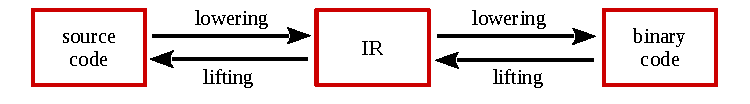
\includegraphics[width=.7\columnwidth]{images/compiler}
  \caption{\label{fig:lowering} Lowering and lifting processes in native vs. source code processing.}
\end{figure}

Reasoning at the intermediate representation level allows program analyses to be written in an architecture-independent fashion. Translated instructions will always expose all the side-effects of a native instruction, and support for additional platforms can be added over time. A number of symbolic executors use VEX, the intermediate representation format from the Valgrind dynamic instrumentation framework~\cite{VALGRIND-PLDI07}. VEX is a RISC-like language designed for program analysis that offers a compact set of instructions for expressing programs in static single assignment (SSA) form. Lifters are available for both 32-bit and 64-bit versions of ARM, MIPS, PPC, and x86 binaries.

~\cite{ANGR-SP16} performs analysis directly on the VEX IR. Authors chose VEX over other IR formats as at that time it was the only choice that offered a publicly available implementation with support for many architectures. Also, they mention that writing a binary lifter can be a daunting task, and a well-documented and program analysis-oriented solution can be a bonus. ~\cite{BITBLAZE-ICISS08} uses VEX too, although it translates it to a custom intermediate language. The reason for this is that VEX captures the side effects of some instructions only implicitly, such as what {\tt EFLAGS} are set by x86 instructions: translating it to a custom language allowed them to simplify the development of their analysis framework.

The authors of ~\cite{CKC-TOCS12} have implemented an x86-to-LLVM-IR lifter in order to use the KLEE symbolic execution engine for whole-system symbolic analysis of binary code in a virtualized environment. The translation is transparent to both the guest operating systems and KLEE, thus allowing them to analyze binaries using the full power of KLEE. Another example of lifter that can be used to run KLEE on binary code is {\tt mcsema}\footnote{\url{https://github.com/trailofbits/mcsema}}.

\subsection{Reconstructing the Control Flow Graph}

\mynote{Motivate first stmt?}Control flow graphs (CFGs) can provide valuable information for a symbolic executor. A fundamental issue that arises when reconstructing CFGs for binaries is that the possible targets of an indirect jump may not be identified correctly. Direct jumps are straightforward to process: as they encode their targets explicitly in the code, successor basic blocks can be identified and visited until no new edge is found. The target of an indirect jump is determined instead at run time: it might be computed by carrying out a calculation (e.g., a jump table) or depend on the current calling context (e.g., a function pointer is passed as argument, or a virtual C++ method is invoked). %We refer the interested reader to ~\cite{ANGR-SP16} for a detailed overview.

In general, not all the analyses based on CFGs require successor nodes to be accurately identified. This property can be exploited to perform further refinements on an initially less accurate CFG using techniques such as Value Set Analysis (VSA)\mynote{VSA cited before}, which require an input CFG themselves. In ~\cite{BITBLAZE-ICISS08} a first version of the CFG is generated by inserting special successor nodes for unresolved indirect jump targets. This choice is conceptually similar to what happens in data-flow analyses when a fact is widened to the bottom of a lattice. When an analysis requires more precise information, VSA is thus applied to the initial CFG.

~\cite{ANGR-SP16} implements two algorithms for CFG recovery. An iterative algorithm starts from the entry point of the program and interleaves a number of techniques to achieve speed and completeness, including VSA, inter-procedural backward program slicing, and symbolic execution of blocks. This algorithm is however rather slow and may miss code portions reachable only through unresolved jump targets. The authors thus devise a fast secondary algorithm that uses a number of heuristics to identify functions based on prologue signatures, and performs simple analyses (e.g., a lightweight alias analysis) to solve a number of indirect jumps. The algorithm is context-insensitive, so it can be used to quickly recover a CFG without a concern for understanding the reachability of functions from one another. 

\subsection{Other Techniques}

\missing\mynote{Types, ...}

\vspace{4em}
\mynote{Notes from D\&E start here} For software such as common off-the-shelf programs, neither users nor attackers have access to their source code: 

Challenges (e.g., ~\cite{BITBLAZE-ICISS08}):
\begin{enumerate}
\item Complexity of the instruction sets
\item Lack of a higher-level semantics (functions/CFG, types, buffers)
\item Obfuscation/dynamic code generation
\end{enumerate}

Symbolic techniques may work on the source code or on the binary code. However, it is not uncommon that both the former and the latter work by reasoning on an intermediate representation of the original code. For instance, ~\cite{KLEE-OSDI08} interprets the LLVM bytecode generated by compiling the source code, while~\cite{ANGR-SP16} reasons on the VEX IR that has been obtained by lifting the binary code.

